\documentclass[border=10pt]{standalone} 
\usepackage{tikz}

\usetikzlibrary{calc}
\usetikzlibrary{arrows}
\usetikzlibrary{shadows}
\usetikzlibrary{patterns}
\usetikzlibrary{positioning}
\usetikzlibrary{shapes}
\usetikzlibrary{3d}
%\usetikzlibrary{automata}
\usetikzlibrary{fit}

\tikzset{block/.style={draw, text centered, fill=gray!10,drop shadow}}
\tikzset{connect/.style={draw, line width=1 pt}}

\begin{document}


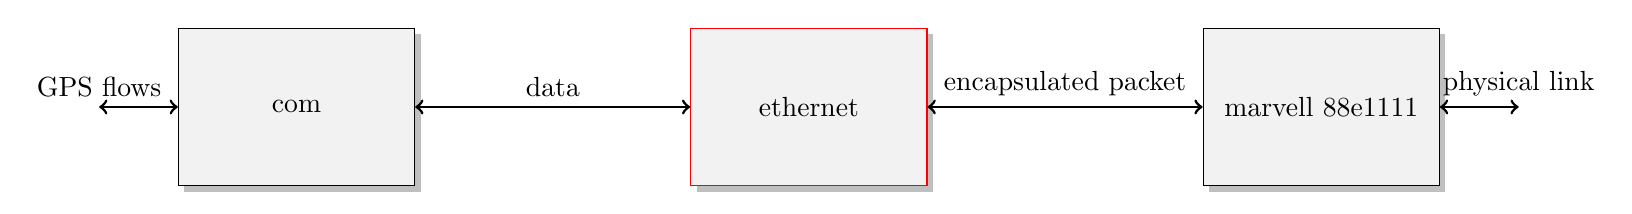
\begin{tikzpicture}

\node[block,minimum height=2cm,minimum width=3cm, draw=red] (eth) {ethernet};
\node[block,minimum height=2cm,minimum width=3cm] (com) at([xshift=-5cm]eth.west){com};
\node[block,minimum height=2cm,minimum width=3cm] (phy) at([xshift=5cm]eth.east) {marvell 88e1111};

\path[connect,<->] (phy.east) --++(1cm,0cm) node[above]{physical link};
\path[connect,<->] (phy.west) -- node[above]{encapsulated packet} (eth.east);
\path[connect,<->] (com.east) -- node[above]{data} (eth.west);
\path[connect,<->] (com.west) --++(-1cm,0cm) node[above]{GPS flows};

\end{tikzpicture}


\end{document}